\documentclass{beamer}
\usepackage[spanish]{babel}
\usepackage{ragged2e}
\usepackage{listings}

\addtobeamertemplate{block begin}{}{\justifying}{}
\apptocmd{\frame}{}{\justifying}{}


\title{Modelado y simulación del Robot Mitsubishi RV-2JA controlado
mediante señales electromiográficas}

\author{
    Busso, Francisco Ignacio \and
    \\ Gautero, Francisco \and
    \\ Gregoret, Guillermo}
\institute{Universidad Tecnológica Nacional\\Facultad Regional Santa Fe}
\date{\today}



\begin{document}

    \begin{frame}
        \titlepage
    \end{frame}

    \begin{frame}
        \frametitle{Valores de Referencia}
        \hspace*{20pt}Para generar valores de cada señal EMG se optó por una distribución uniforme con 
        variación del 5\% sobre las señales de referencia.
        \begin{figure}
            \centering
            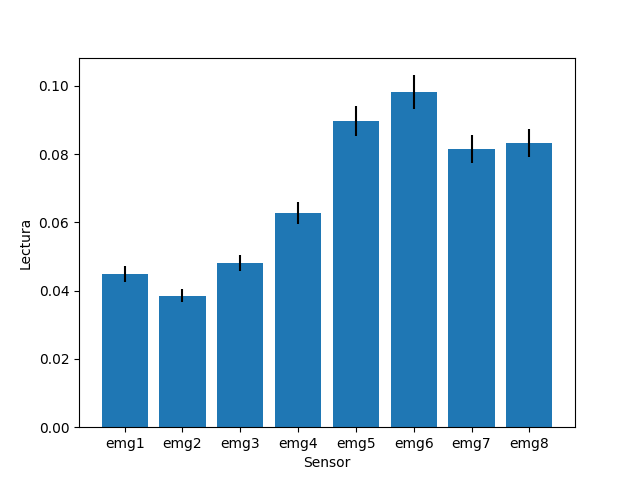
\includegraphics[scale=0.4]{plot.png}
            \caption{Valores de Referencia para cada sensor}
        \end{figure}
    \end{frame} 

    \begin{frame}
        \frametitle{Etiquetado del Set de Datos}
        \hspace*{20pt}Se define un valor umbral para determinar si el valor de la lectura de un sensor pertenece a los valores admitidos.
        \vspace*{5pt}
        \lstinputlisting[language=Python, firstline=1, lastline=3, basicstyle=\tiny]{snippets.txt}
        \vspace*{10pt}
        \hspace*{20pt}Si las lecturas de todos los sensores se encuentran dentro del rango admitido, la entrada se etiqueta como 1; si no, se etiqueta como 0.
        \vspace*{5pt}
        \lstinputlisting[language=Python, firstline=5, lastline=6, basicstyle=\tiny]{snippets.txt}
    \end{frame} 

    \begin{frame}
        \frametitle{Obtención del Set de Entrenamiento}
        \hspace*{20pt}Se lee un set de datos, se lo etiqueta y se lo separa entre un set de entrenamiento y un set de pruebas.
        \vspace*{10pt}
        \lstinputlisting[language=Python, firstline=8, lastline=16, basicstyle=\tiny]{snippets.txt}

    \end{frame}   


    \begin{frame}
        \frametitle{Implementación con scikit-learn}

        \hspace*{20pt}La clase MLPClassifier implementa un algoritmo de entrenamiento de perceptrón 
        multicapa \textit{(MLP)} utilizando propagación hacia atrás \textit{(Backpropagation)}.
        \vspace*{10pt}
        \lstinputlisting[language=Python, firstline=18, lastline=21, basicstyle=\tiny]{snippets.txt}



    \end{frame}

    \begin{frame}
        \frametitle{El Algoritmo MLP}
        \hspace*{20pt}El algoritmo toma como entrada dos arreglos: $X$, de dimensiones ($n-muestras$, $n-caracteristicas$), 
        que representa las muestras de entrenamiento como vectores de punto flotante; e $Y$ de tamaño ($n-muestras$), 
        que almacena los valores de las etiquetas de clase para las muestras de entrenamiento.
        \vspace*{10pt}
        \lstinputlisting[language=Python, firstline=23, lastline=26, basicstyle=\scriptsize]{snippets.txt}


    \end{frame}

    \begin{frame}
        \frametitle{Predicciones}

        \hspace*{20pt}Luego del ajuste (entrenamiento), el modelo puede predecir las etiquetas para nuevas muestras
        \vspace*{10pt}
        \lstinputlisting[language=Python, firstline=28, lastline=29, basicstyle=\scriptsize]{snippets.txt}

    \end{frame}

    \begin{frame}
        \frametitle{Similitud Coseno}

        \hspace*{20pt}Es una medida de la similitud existente entre dos vectores en un espacio multidimensional 
        (más precisamente un espacio \textit{pre-hilbertiano}) con el que se evalúa el valor del coseno del ángulo comprendido 
        entre ellos.\\~\

        \hspace*{20pt}Proporciona un valor igual a 1 si el ángulo comprendido es cero. Cualquier ángulo existente entre los vectores, 
        el coseno arrojaría un valor inferior a uno. \\~\

        \hspace*{20pt}\textit{\scriptsize{La similitud coseno no debe ser considerada como una métrica debido a que no cumple la desigualdad triangular.}}
    \end{frame}

    \begin{frame}
        \frametitle{Complejidad de la Solución}

        \hspace*{20pt}Suponiendo $n$ muestras de entrenamiento, $m$ características, $k$ capas ocultas cada una conteniendo $h$ 
        neuronas y, para simplificar, o neuronas en la capa de salida. La complejidad temporal de la propagación hacia atrás es 
        $O(n*m*h^k*o*i)$, donde $i$ es el número de iteraciones.\\~\
        
        \hspace*{20pt}Dado que el método de \text{Backpropagation} tiene alta complejidad temporal, es recomendable comenzar con un número 
        bajo de neuronas en la capa oculta para el entrenamiento.

    \end{frame}  

    \begin{frame}
        \frametitle{Escalabilidad de la Solución}

        \hspace*{20pt}Esta implementación no está pensada para aplicaciones de gran escala. 
        En particular, scikit-learn no ofrece soporte para GPU.


    \end{frame}  



\end{document}